\documentclass[1p]{elsarticle_modified}
%\bibliographystyle{elsarticle-num}

%\usepackage[colorlinks]{hyperref}
%\usepackage{abbrmath_seonhwa} %\Abb, \Ascr, \Acal ,\Abf, \Afrak
\usepackage{amsfonts}
\usepackage{amssymb}
\usepackage{amsmath}
\usepackage{amsthm}
\usepackage{scalefnt}
\usepackage{amsbsy}
\usepackage{kotex}
\usepackage{caption}
\usepackage{subfig}
\usepackage{color}
\usepackage{graphicx}
\usepackage{xcolor} %% white, black, red, green, blue, cyan, magenta, yellow
\usepackage{float}
\usepackage{setspace}
\usepackage{hyperref}

\usepackage{tikz}
\usetikzlibrary{arrows}

\usepackage{multirow}
\usepackage{array} % fixed length table
\usepackage{hhline}

%%%%%%%%%%%%%%%%%%%%%
\makeatletter
\renewcommand*\env@matrix[1][\arraystretch]{%
	\edef\arraystretch{#1}%
	\hskip -\arraycolsep
	\let\@ifnextchar\new@ifnextchar
	\array{*\c@MaxMatrixCols c}}
\makeatother %https://tex.stackexchange.com/questions/14071/how-can-i-increase-the-line-spacing-in-a-matrix
%%%%%%%%%%%%%%%

\usepackage[normalem]{ulem}

\newcommand{\msout}[1]{\ifmmode\text{\sout{\ensuremath{#1}}}\else\sout{#1}\fi}
%SOURCE: \msout is \stkout macro in https://tex.stackexchange.com/questions/20609/strikeout-in-math-mode

\newcommand{\cancel}[1]{
	\ifmmode
	{\color{red}\msout{#1}}
	\else
	{\color{red}\sout{#1}}
	\fi
}

\newcommand{\add}[1]{
	{\color{blue}\uwave{#1}}
}

\newcommand{\replace}[2]{
	\ifmmode
	{\color{red}\msout{#1}}{\color{blue}\uwave{#2}}
	\else
	{\color{red}\sout{#1}}{\color{blue}\uwave{#2}}
	\fi
}

\newcommand{\Sol}{\mathcal{S}} %segment
\newcommand{\D}{D} %diagram
\newcommand{\A}{\mathcal{A}} %arc


%%%%%%%%%%%%%%%%%%%%%%%%%%%%%5 test

\def\sl{\operatorname{\textup{SL}}(2,\Cbb)}
\def\psl{\operatorname{\textup{PSL}}(2,\Cbb)}
\def\quan{\mkern 1mu \triangleright \mkern 1mu}

\theoremstyle{definition}
\newtheorem{thm}{Theorem}[section]
\newtheorem{prop}[thm]{Proposition}
\newtheorem{lem}[thm]{Lemma}
\newtheorem{ques}[thm]{Question}
\newtheorem{cor}[thm]{Corollary}
\newtheorem{defn}[thm]{Definition}
\newtheorem{exam}[thm]{Example}
\newtheorem{rmk}[thm]{Remark}
\newtheorem{alg}[thm]{Algorithm}

\newcommand{\I}{\sqrt{-1}}
\begin{document}

%\begin{frontmatter}
%
%\title{Boundary parabolic representations of knots up to 8 crossings}
%
%%% Group authors per affiliation:
%\author{Yunhi Cho} 
%\address{Department of Mathematics, University of Seoul, Seoul, Korea}
%\ead{yhcho@uos.ac.kr}
%
%
%\author{Seonhwa Kim} %\fnref{s_kim}}
%\address{Center for Geometry and Physics, Institute for Basic Science, Pohang, 37673, Korea}
%\ead{ryeona17@ibs.re.kr}
%
%\author{Hyuk Kim}
%\address{Department of Mathematical Sciences, Seoul National University, Seoul 08826, Korea}
%\ead{hyukkim@snu.ac.kr}
%
%\author{Seokbeom Yoon}
%\address{Department of Mathematical Sciences, Seoul National University, Seoul, 08826,  Korea}
%\ead{sbyoon15@snu.ac.kr}
%
%\begin{abstract}
%We find all boundary parabolic representation of knots up to 8 crossings.
%
%\end{abstract}
%\begin{keyword}
%    \MSC[2010] 57M25 
%\end{keyword}
%
%\end{frontmatter}

%\linenumbers
%\tableofcontents
%
\newcommand\colored[1]{\textcolor{white}{\rule[-0.35ex]{0.8em}{1.4ex}}\kern-0.8em\color{red} #1}%
%\newcommand\colored[1]{\textcolor{white}{ #1}\kern-2.17ex	\textcolor{white}{ #1}\kern-1.81ex	\textcolor{white}{ #1}\kern-2.15ex\color{red}#1	}

{\Large $\underline{12a_{1259}~(K12a_{1259})}$}

\setlength{\tabcolsep}{10pt}
\renewcommand{\arraystretch}{1.6}
\vspace{1cm}\begin{tabular}{m{100pt}>{\centering\arraybackslash}m{274pt}}
\multirow{5}{120pt}{
	\centering
	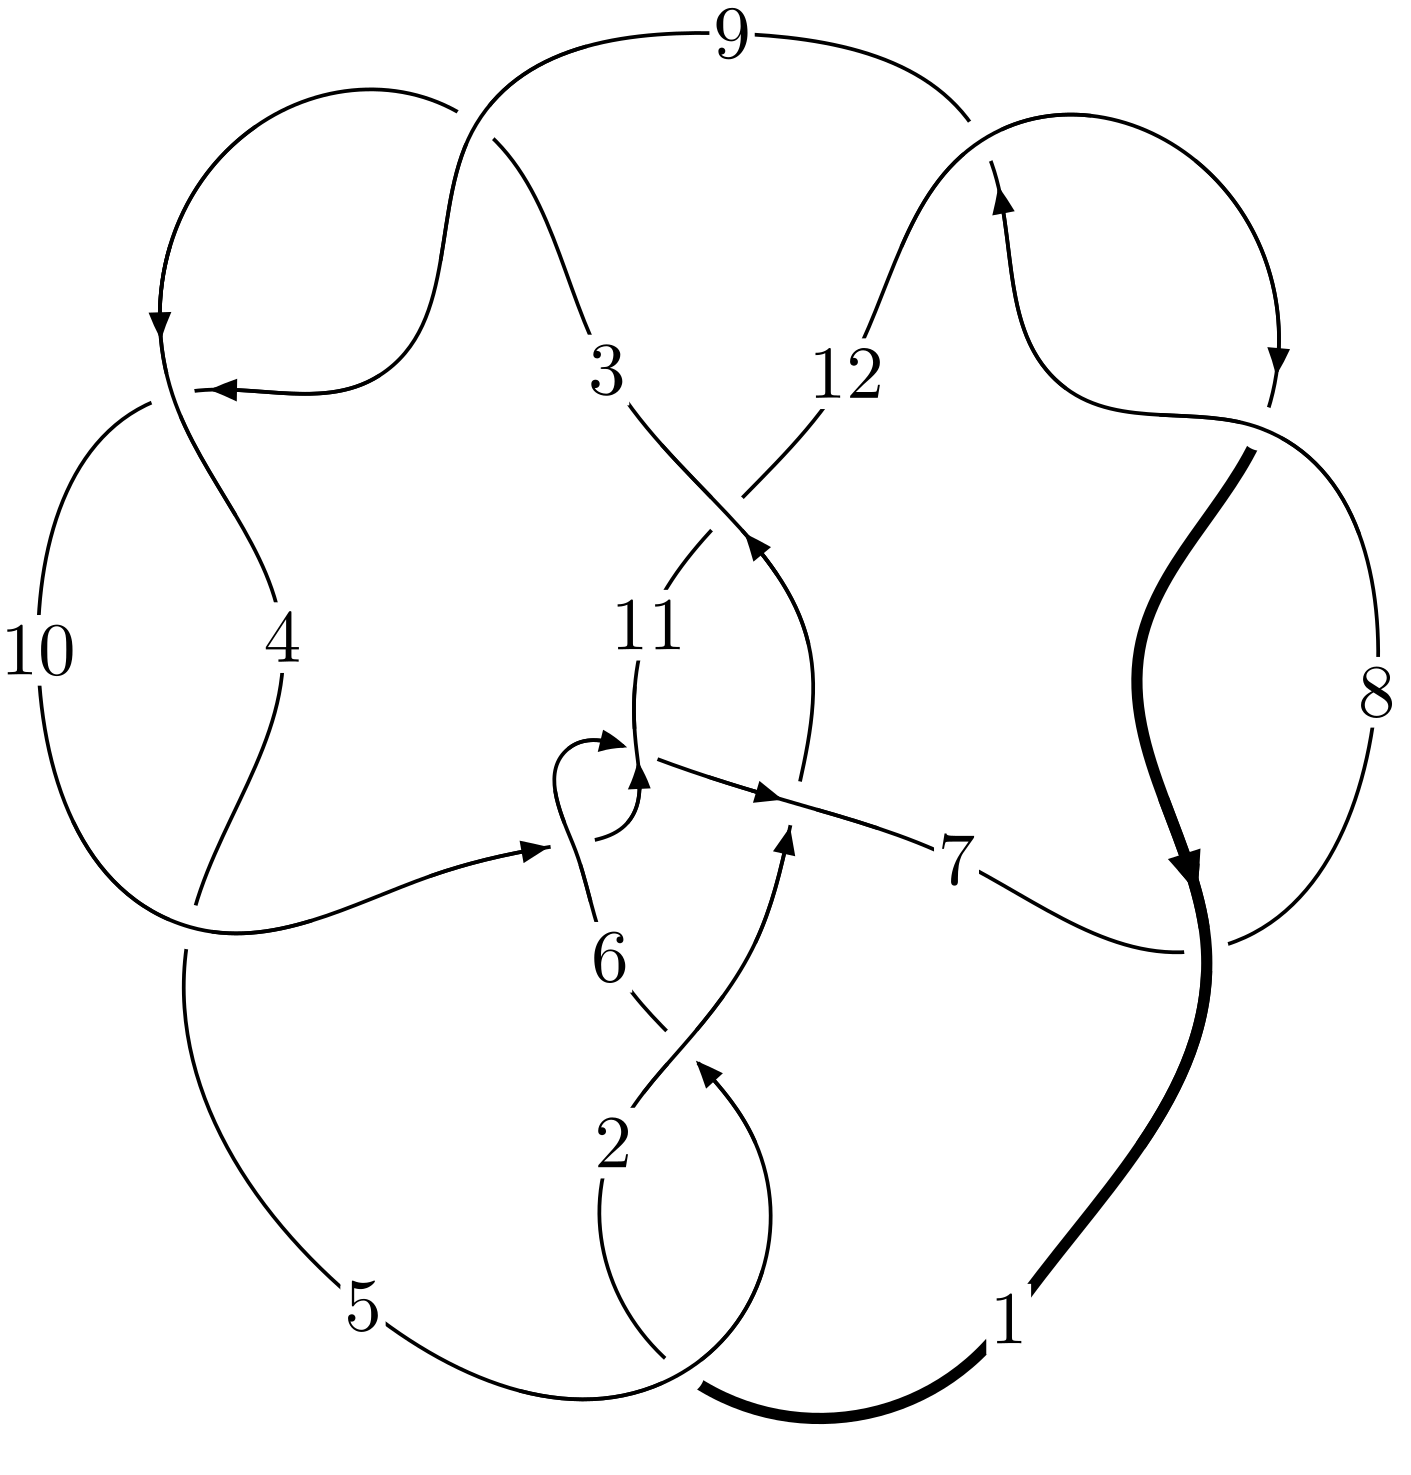
\includegraphics[width=112pt]{../../../GIT/diagram.site/Diagrams/png/2060_12a_1259.png}\\
\ \ \ A knot diagram\footnotemark}&
\allowdisplaybreaks
\textbf{Linearized knot diagam} \\
\cline{2-2}
 &
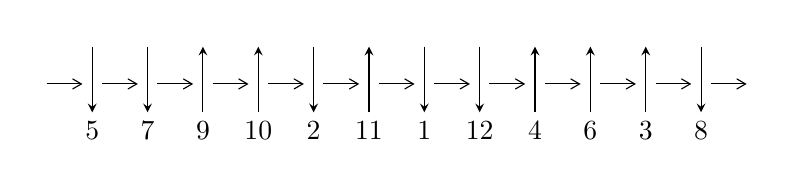
\begin{tikzpicture}[x=20pt, y=17pt]
	% nodes
	\node (C0) at (0, 0) {};
	\node (C1) at (1, 0) {};
	\node (C1U) at (1, +1) {};
	\node (C1D) at (1, -1) {5};

	\node (C2) at (2, 0) {};
	\node (C2U) at (2, +1) {};
	\node (C2D) at (2, -1) {7};

	\node (C3) at (3, 0) {};
	\node (C3U) at (3, +1) {};
	\node (C3D) at (3, -1) {9};

	\node (C4) at (4, 0) {};
	\node (C4U) at (4, +1) {};
	\node (C4D) at (4, -1) {10};

	\node (C5) at (5, 0) {};
	\node (C5U) at (5, +1) {};
	\node (C5D) at (5, -1) {2};

	\node (C6) at (6, 0) {};
	\node (C6U) at (6, +1) {};
	\node (C6D) at (6, -1) {11};

	\node (C7) at (7, 0) {};
	\node (C7U) at (7, +1) {};
	\node (C7D) at (7, -1) {1};

	\node (C8) at (8, 0) {};
	\node (C8U) at (8, +1) {};
	\node (C8D) at (8, -1) {12};

	\node (C9) at (9, 0) {};
	\node (C9U) at (9, +1) {};
	\node (C9D) at (9, -1) {4};

	\node (C10) at (10, 0) {};
	\node (C10U) at (10, +1) {};
	\node (C10D) at (10, -1) {6};

	\node (C11) at (11, 0) {};
	\node (C11U) at (11, +1) {};
	\node (C11D) at (11, -1) {3};

	\node (C12) at (12, 0) {};
	\node (C12U) at (12, +1) {};
	\node (C12D) at (12, -1) {8};
	\node (C13) at (13, 0) {};

	% arrows
	\draw[->,>={angle 60}]
	(C0) edge (C1) (C1) edge (C2) (C2) edge (C3) (C3) edge (C4) (C4) edge (C5) (C5) edge (C6) (C6) edge (C7) (C7) edge (C8) (C8) edge (C9) (C9) edge (C10) (C10) edge (C11) (C11) edge (C12) (C12) edge (C13) ;	\draw[->,>=stealth]
	(C1U) edge (C1D) (C2U) edge (C2D) (C3D) edge (C3U) (C4D) edge (C4U) (C5U) edge (C5D) (C6D) edge (C6U) (C7U) edge (C7D) (C8U) edge (C8D) (C9D) edge (C9U) (C10D) edge (C10U) (C11D) edge (C11U) (C12U) edge (C12D) ;
	\end{tikzpicture} \\
\hhline{~~} \\& 
\textbf{Solving Sequence} \\ \cline{2-2} 
 &
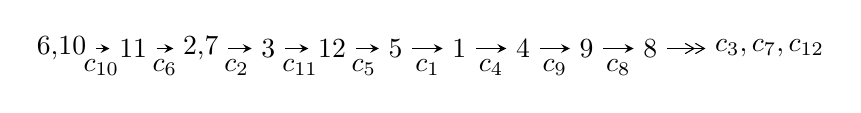
\begin{tikzpicture}[x=23pt, y=7pt]
	% node
	\node (A0) at (-1/8, 0) {6,10};
	\node (A1) at (1, 0) {11};
	\node (A2) at (33/16, 0) {2,7};
	\node (A3) at (25/8, 0) {3};
	\node (A4) at (33/8, 0) {12};
	\node (A5) at (41/8, 0) {5};
	\node (A6) at (49/8, 0) {1};
	\node (A7) at (57/8, 0) {4};
	\node (A8) at (65/8, 0) {9};
	\node (A9) at (73/8, 0) {8};
	\node (C1) at (1/2, -1) {$c_{10}$};
	\node (C2) at (3/2, -1) {$c_{6}$};
	\node (C3) at (21/8, -1) {$c_{2}$};
	\node (C4) at (29/8, -1) {$c_{11}$};
	\node (C5) at (37/8, -1) {$c_{5}$};
	\node (C6) at (45/8, -1) {$c_{1}$};
	\node (C7) at (53/8, -1) {$c_{4}$};
	\node (C8) at (61/8, -1) {$c_{9}$};
	\node (C9) at (69/8, -1) {$c_{8}$};
	\node (A10) at (11, 0) {$c_{3},c_{7},c_{12}$};

	% edge
	\draw[->,>=stealth]	
	(A0) edge (A1) (A1) edge (A2) (A2) edge (A3) (A3) edge (A4) (A4) edge (A5) (A5) edge (A6) (A6) edge (A7) (A7) edge (A8) (A8) edge (A9) ;
	\draw[->>,>={angle 60}]	
	(A9) edge (A10);
\end{tikzpicture} \\ 

\end{tabular} \\

\footnotetext{
The image of knot diagram is generated by the software ``\textbf{Draw programme}" developed by Andrew Bartholomew(\url{http://www.layer8.co.uk/maths/draw/index.htm\#Running-draw}), where we modified some parts for our purpose(\url{https://github.com/CATsTAILs/LinksPainter}).
}\phantom \\ \newline 
\centering \textbf{Ideals for irreducible components\footnotemark of $X_{\text{par}}$} 
 
\begin{align*}
I^u_{1}&=\langle 
5.69308\times10^{303} u^{97}-1.06736\times10^{304} u^{96}+\cdots+4.39641\times10^{304} b+1.65833\times10^{306},\\
\phantom{I^u_{1}}&\phantom{= \langle  }-1.21815\times10^{306} u^{97}-1.21298\times10^{306} u^{96}+\cdots+3.47317\times10^{306} a+1.09802\times10^{308},\\
\phantom{I^u_{1}}&\phantom{= \langle  }u^{98}+u^{97}+\cdots-192 u+79\rangle \\
I^u_{2}&=\langle 
-1240865 u^{26}+78914 u^{25}+\cdots+933437 b+295188,\\
\phantom{I^u_{2}}&\phantom{= \langle  }-8955091 u^{26}-9064939 u^{25}+\cdots+933437 a-23614626,\;u^{27}-9 u^{25}+\cdots+9 u^2-1\rangle \\
\\
\end{align*}
\raggedright * 2 irreducible components of $\dim_{\mathbb{C}}=0$, with total 125 representations.\\
\footnotetext{All coefficients of polynomials are rational numbers. But the coefficients are sometimes approximated in decimal forms when there is not enough margin.}
\newpage
\renewcommand{\arraystretch}{1}
\centering \section*{I. $I^u_{1}= \langle 5.69\times10^{303} u^{97}-1.07\times10^{304} u^{96}+\cdots+4.40\times10^{304} b+1.66\times10^{306},\;-1.22\times10^{306} u^{97}-1.21\times10^{306} u^{96}+\cdots+3.47\times10^{306} a+1.10\times10^{308},\;u^{98}+u^{97}+\cdots-192 u+79 \rangle$}
\flushleft \textbf{(i) Arc colorings}\\
\begin{tabular}{m{7pt} m{180pt} m{7pt} m{180pt} }
\flushright $a_{6}=$&$\begin{pmatrix}0\\u\end{pmatrix}$ \\
\flushright $a_{10}=$&$\begin{pmatrix}1\\0\end{pmatrix}$ \\
\flushright $a_{11}=$&$\begin{pmatrix}1\\- u^2\end{pmatrix}$ \\
\flushright $a_{2}=$&$\begin{pmatrix}0.350731 u^{97}+0.349244 u^{96}+\cdots+34.5787 u-31.6144\\-0.129494 u^{97}+0.242779 u^{96}+\cdots+63.5735 u-37.7201\end{pmatrix}$ \\
\flushright $a_{7}=$&$\begin{pmatrix}u\\- u^3+u\end{pmatrix}$ \\
\flushright $a_{3}=$&$\begin{pmatrix}0.635075 u^{97}+0.290148 u^{96}+\cdots-26.8955 u-14.5431\\-0.154509 u^{97}+0.303320 u^{96}+\cdots+90.5028 u-47.7805\end{pmatrix}$ \\
\flushright $a_{12}=$&$\begin{pmatrix}-0.279601 u^{97}-0.295570 u^{96}+\cdots+17.3434 u+33.7179\\-0.0375579 u^{97}-0.0703430 u^{96}+\cdots-8.10495 u+0.408463\end{pmatrix}$ \\
\flushright $a_{5}=$&$\begin{pmatrix}0.223768 u^{97}+0.576551 u^{96}+\cdots+72.9539 u-63.0265\\0.0190934 u^{97}-0.103748 u^{96}+\cdots-38.7659 u+19.0595\end{pmatrix}$ \\
\flushright $a_{1}=$&$\begin{pmatrix}0.0147025 u^{97}-0.0896428 u^{96}+\cdots-44.5524 u+43.9400\\0.0261589 u^{97}-0.0145128 u^{96}+\cdots-28.2070 u+1.37104\end{pmatrix}$ \\
\flushright $a_{4}=$&$\begin{pmatrix}0.204674 u^{97}+0.680299 u^{96}+\cdots+111.720 u-82.0860\\0.0190934 u^{97}-0.103748 u^{96}+\cdots-38.7659 u+19.0595\end{pmatrix}$ \\
\flushright $a_{9}=$&$\begin{pmatrix}-0.289035 u^{97}+0.180873 u^{96}+\cdots+111.655 u-64.0028\\0.140591 u^{97}-0.182545 u^{96}+\cdots-76.3010 u+39.1583\end{pmatrix}$ \\
\flushright $a_{8}=$&$\begin{pmatrix}-0.136447 u^{97}+0.413129 u^{96}+\cdots+145.083 u-58.1068\\0.238402 u^{97}+0.490572 u^{96}+\cdots+48.6728 u-44.2169\end{pmatrix}$\\&\end{tabular}
\flushleft \textbf{(ii) Obstruction class $= -1$}\\~\\
\flushleft \textbf{(iii) Cusp Shapes $= -1.47472 u^{97}-1.63887 u^{96}+\cdots+179.736 u+58.6258$}\\~\\
\newpage\renewcommand{\arraystretch}{1}
\flushleft \textbf{(iv) u-Polynomials at the component}\newline \\
\begin{tabular}{m{50pt}|m{274pt}}
Crossings & \hspace{64pt}u-Polynomials at each crossing \\
\hline $$\begin{aligned}c_{1},c_{5}\end{aligned}$$&$\begin{aligned}
&u^{98}-24 u^{96}+\cdots+179 u-49
\end{aligned}$\\
\hline $$\begin{aligned}c_{2}\end{aligned}$$&$\begin{aligned}
&u^{98}- u^{97}+\cdots-175987 u-451
\end{aligned}$\\
\hline $$\begin{aligned}c_{3},c_{4},c_{9}\end{aligned}$$&$\begin{aligned}
&u^{98}- u^{97}+\cdots-224 u-32
\end{aligned}$\\
\hline $$\begin{aligned}c_{6},c_{10}\end{aligned}$$&$\begin{aligned}
&u^{98}+u^{97}+\cdots-192 u+79
\end{aligned}$\\
\hline $$\begin{aligned}c_{7},c_{8},c_{12}\end{aligned}$$&$\begin{aligned}
&u^{98}+2 u^{97}+\cdots-36 u+19
\end{aligned}$\\
\hline $$\begin{aligned}c_{11}\end{aligned}$$&$\begin{aligned}
&u^{98}-5 u^{97}+\cdots-215663520 u+43957163
\end{aligned}$\\
\hline
\end{tabular}\\~\\
\newpage\renewcommand{\arraystretch}{1}
\flushleft \textbf{(v) Riley Polynomials at the component}\newline \\
\begin{tabular}{m{50pt}|m{274pt}}
Crossings & \hspace{64pt}Riley Polynomials at each crossing \\
\hline $$\begin{aligned}c_{1},c_{5}\end{aligned}$$&$\begin{aligned}
&y^{98}-48 y^{97}+\cdots-56639 y+2401
\end{aligned}$\\
\hline $$\begin{aligned}c_{2}\end{aligned}$$&$\begin{aligned}
&y^{98}+23 y^{97}+\cdots-31146246201 y+203401
\end{aligned}$\\
\hline $$\begin{aligned}c_{3},c_{4},c_{9}\end{aligned}$$&$\begin{aligned}
&y^{98}-109 y^{97}+\cdots-160768 y+1024
\end{aligned}$\\
\hline $$\begin{aligned}c_{6},c_{10}\end{aligned}$$&$\begin{aligned}
&y^{98}-67 y^{97}+\cdots-74626 y+6241
\end{aligned}$\\
\hline $$\begin{aligned}c_{7},c_{8},c_{12}\end{aligned}$$&$\begin{aligned}
&y^{98}+106 y^{97}+\cdots+12536 y+361
\end{aligned}$\\
\hline $$\begin{aligned}c_{11}\end{aligned}$$&$\begin{aligned}
&y^{98}-57 y^{97}+\cdots-68808164574318740 y+1932232179008569
\end{aligned}$\\
\hline
\end{tabular}\\~\\
\newpage\flushleft \textbf{(vi) Complex Volumes and Cusp Shapes}
$$\begin{array}{c|c|c}  
\text{Solutions to }I^u_{1}& \I (\text{vol} + \sqrt{-1}CS) & \text{Cusp shape}\\
 \hline 
\begin{aligned}
u &= -0.147644 + 0.991105 I \\
a &= \phantom{-}0.428223 + 0.979194 I \\
b &= -0.083114 + 1.402650 I\end{aligned}
 & -2.74725 + 3.13007 I & \phantom{-0.000000 } 0 \\ \hline\begin{aligned}
u &= -0.147644 - 0.991105 I \\
a &= \phantom{-}0.428223 - 0.979194 I \\
b &= -0.083114 - 1.402650 I\end{aligned}
 & -2.74725 - 3.13007 I & \phantom{-0.000000 } 0 \\ \hline\begin{aligned}
u &= -0.580157 + 0.788031 I \\
a &= \phantom{-}1.330990 + 0.437564 I \\
b &= \phantom{-}0.250861 + 0.849982 I\end{aligned}
 & \phantom{-}8.50650 + 1.10397 I & \phantom{-0.000000 } 0 \\ \hline\begin{aligned}
u &= -0.580157 - 0.788031 I \\
a &= \phantom{-}1.330990 - 0.437564 I \\
b &= \phantom{-}0.250861 - 0.849982 I\end{aligned}
 & \phantom{-}8.50650 - 1.10397 I & \phantom{-0.000000 } 0 \\ \hline\begin{aligned}
u &= \phantom{-}0.969739 + 0.067480 I \\
a &= \phantom{-}0.855963 - 0.493667 I \\
b &= -0.64297 - 1.34543 I\end{aligned}
 & \phantom{-}1.110890 + 0.358653 I & \phantom{-0.000000 } 0 \\ \hline\begin{aligned}
u &= \phantom{-}0.969739 - 0.067480 I \\
a &= \phantom{-}0.855963 + 0.493667 I \\
b &= -0.64297 + 1.34543 I\end{aligned}
 & \phantom{-}1.110890 - 0.358653 I & \phantom{-0.000000 } 0 \\ \hline\begin{aligned}
u &= -0.982662 + 0.303550 I \\
a &= -0.744825 - 0.890821 I \\
b &= \phantom{-}0.325588 - 1.109070 I\end{aligned}
 & -0.64154 - 2.71485 I & \phantom{-0.000000 } 0 \\ \hline\begin{aligned}
u &= -0.982662 - 0.303550 I \\
a &= -0.744825 + 0.890821 I \\
b &= \phantom{-}0.325588 + 1.109070 I\end{aligned}
 & -0.64154 + 2.71485 I & \phantom{-0.000000 } 0 \\ \hline\begin{aligned}
u &= \phantom{-}1.02854\phantom{ +0.000000I} \\
a &= -1.64694\phantom{ +0.000000I} \\
b &= \phantom{-}1.45660\phantom{ +0.000000I}\end{aligned}
 & \phantom{-}2.65903\phantom{ +0.000000I} & \phantom{-0.000000 } 0 \\ \hline\begin{aligned}
u &= -1.031350 + 0.102678 I \\
a &= \phantom{-}1.39462 + 0.63971 I \\
b &= -1.40148 + 0.67569 I\end{aligned}
 & \phantom{-}6.05602 - 4.27471 I & \phantom{-0.000000 } 0\\
 \hline 
 \end{array}$$\newpage$$\begin{array}{c|c|c}  
\text{Solutions to }I^u_{1}& \I (\text{vol} + \sqrt{-1}CS) & \text{Cusp shape}\\
 \hline 
\begin{aligned}
u &= -1.031350 - 0.102678 I \\
a &= \phantom{-}1.39462 - 0.63971 I \\
b &= -1.40148 - 0.67569 I\end{aligned}
 & \phantom{-}6.05602 + 4.27471 I & \phantom{-0.000000 } 0 \\ \hline\begin{aligned}
u &= -1.017430 + 0.216044 I \\
a &= \phantom{-}1.07032 + 0.98555 I \\
b &= -1.17396 + 1.08732 I\end{aligned}
 & \phantom{-}6.07548 - 4.43283 I & \phantom{-0.000000 } 0 \\ \hline\begin{aligned}
u &= -1.017430 - 0.216044 I \\
a &= \phantom{-}1.07032 - 0.98555 I \\
b &= -1.17396 - 1.08732 I\end{aligned}
 & \phantom{-}6.07548 + 4.43283 I & \phantom{-0.000000 } 0 \\ \hline\begin{aligned}
u &= \phantom{-}0.951483 + 0.470279 I \\
a &= -0.460130 + 1.277270 I \\
b &= \phantom{-}0.81690 + 1.41346 I\end{aligned}
 & \phantom{-}3.57337 + 5.44735 I & \phantom{-0.000000 } 0 \\ \hline\begin{aligned}
u &= \phantom{-}0.951483 - 0.470279 I \\
a &= -0.460130 - 1.277270 I \\
b &= \phantom{-}0.81690 - 1.41346 I\end{aligned}
 & \phantom{-}3.57337 - 5.44735 I & \phantom{-0.000000 } 0 \\ \hline\begin{aligned}
u &= \phantom{-}1.059930 + 0.107788 I \\
a &= -0.638112 - 0.319931 I \\
b &= \phantom{-}0.186539 - 0.221069 I\end{aligned}
 & \phantom{-}2.11130 + 0.19001 I & \phantom{-0.000000 } 0 \\ \hline\begin{aligned}
u &= \phantom{-}1.059930 - 0.107788 I \\
a &= -0.638112 + 0.319931 I \\
b &= \phantom{-}0.186539 + 0.221069 I\end{aligned}
 & \phantom{-}2.11130 - 0.19001 I & \phantom{-0.000000 } 0 \\ \hline\begin{aligned}
u &= -1.066920 + 0.069450 I \\
a &= -0.649537 + 0.367157 I \\
b &= \phantom{-}0.70174 + 1.97988 I\end{aligned}
 & \phantom{-}8.50659 - 0.46621 I & \phantom{-0.000000 } 0 \\ \hline\begin{aligned}
u &= -1.066920 - 0.069450 I \\
a &= -0.649537 - 0.367157 I \\
b &= \phantom{-}0.70174 - 1.97988 I\end{aligned}
 & \phantom{-}8.50659 + 0.46621 I & \phantom{-0.000000 } 0 \\ \hline\begin{aligned}
u &= -0.022975 + 0.918534 I \\
a &= -0.469657 + 1.282630 I \\
b &= -0.074903 + 1.400880 I\end{aligned}
 & \phantom{-}3.25898 - 6.63136 I & \phantom{-0.000000 } 0\\
 \hline 
 \end{array}$$\newpage$$\begin{array}{c|c|c}  
\text{Solutions to }I^u_{1}& \I (\text{vol} + \sqrt{-1}CS) & \text{Cusp shape}\\
 \hline 
\begin{aligned}
u &= -0.022975 - 0.918534 I \\
a &= -0.469657 - 1.282630 I \\
b &= -0.074903 - 1.400880 I\end{aligned}
 & \phantom{-}3.25898 + 6.63136 I & \phantom{-0.000000 } 0 \\ \hline\begin{aligned}
u &= -0.952127 + 0.513412 I \\
a &= \phantom{-}1.125300 + 0.318980 I \\
b &= \phantom{-}0.042890 + 0.753251 I\end{aligned}
 & \phantom{-}6.32720 + 2.24621 I & \phantom{-0.000000 } 0 \\ \hline\begin{aligned}
u &= -0.952127 - 0.513412 I \\
a &= \phantom{-}1.125300 - 0.318980 I \\
b &= \phantom{-}0.042890 - 0.753251 I\end{aligned}
 & \phantom{-}6.32720 - 2.24621 I & \phantom{-0.000000 } 0 \\ \hline\begin{aligned}
u &= \phantom{-}1.042950 + 0.359828 I \\
a &= \phantom{-}0.521935 - 1.141640 I \\
b &= -0.284407 - 0.974890 I\end{aligned}
 & \phantom{-}3.77548 + 4.91175 I & \phantom{-0.000000 } 0 \\ \hline\begin{aligned}
u &= \phantom{-}1.042950 - 0.359828 I \\
a &= \phantom{-}0.521935 + 1.141640 I \\
b &= -0.284407 + 0.974890 I\end{aligned}
 & \phantom{-}3.77548 - 4.91175 I & \phantom{-0.000000 } 0 \\ \hline\begin{aligned}
u &= -0.935588 + 0.596452 I \\
a &= \phantom{-}0.209599 + 1.336450 I \\
b &= -0.71696 + 1.50993 I\end{aligned}
 & \phantom{-}9.56242 - 6.26495 I & \phantom{-0.000000 } 0 \\ \hline\begin{aligned}
u &= -0.935588 - 0.596452 I \\
a &= \phantom{-}0.209599 - 1.336450 I \\
b &= -0.71696 - 1.50993 I\end{aligned}
 & \phantom{-}9.56242 + 6.26495 I & \phantom{-0.000000 } 0 \\ \hline\begin{aligned}
u &= \phantom{-}0.283477 + 0.837190 I \\
a &= \phantom{-}0.918914 - 0.242800 I \\
b &= \phantom{-}0.12959 - 1.63928 I\end{aligned}
 & \phantom{-}12.78970 + 4.85078 I & \phantom{-0.000000 } 0 \\ \hline\begin{aligned}
u &= \phantom{-}0.283477 - 0.837190 I \\
a &= \phantom{-}0.918914 + 0.242800 I \\
b &= \phantom{-}0.12959 + 1.63928 I\end{aligned}
 & \phantom{-}12.78970 - 4.85078 I & \phantom{-0.000000 } 0 \\ \hline\begin{aligned}
u &= -1.106800 + 0.279137 I \\
a &= \phantom{-}0.394983 - 0.594836 I \\
b &= -0.048083 - 0.550544 I\end{aligned}
 & \phantom{-}3.25698 - 3.46925 I & \phantom{-0.000000 } 0\\
 \hline 
 \end{array}$$\newpage$$\begin{array}{c|c|c}  
\text{Solutions to }I^u_{1}& \I (\text{vol} + \sqrt{-1}CS) & \text{Cusp shape}\\
 \hline 
\begin{aligned}
u &= -1.106800 - 0.279137 I \\
a &= \phantom{-}0.394983 + 0.594836 I \\
b &= -0.048083 + 0.550544 I\end{aligned}
 & \phantom{-}3.25698 + 3.46925 I & \phantom{-0.000000 } 0 \\ \hline\begin{aligned}
u &= -0.531479 + 0.670358 I \\
a &= -0.612662 - 1.101300 I \\
b &= \phantom{-}1.26914 - 0.84801 I\end{aligned}
 & \phantom{-}0.93590 - 2.76801 I & \phantom{-0.000000 } 0 \\ \hline\begin{aligned}
u &= -0.531479 - 0.670358 I \\
a &= -0.612662 + 1.101300 I \\
b &= \phantom{-}1.26914 + 0.84801 I\end{aligned}
 & \phantom{-}0.93590 + 2.76801 I & \phantom{-0.000000 } 0 \\ \hline\begin{aligned}
u &= \phantom{-}0.594310 + 0.611420 I \\
a &= -1.351400 + 0.376376 I \\
b &= -0.248207 + 0.834678 I\end{aligned}
 & \phantom{-}2.54743 - 1.15983 I & \phantom{-0.000000 } 0 \\ \hline\begin{aligned}
u &= \phantom{-}0.594310 - 0.611420 I \\
a &= -1.351400 - 0.376376 I \\
b &= -0.248207 - 0.834678 I\end{aligned}
 & \phantom{-}2.54743 + 1.15983 I & \phantom{-0.000000 } 0 \\ \hline\begin{aligned}
u &= -1.165460 + 0.037280 I \\
a &= \phantom{-}0.888037 - 0.660491 I \\
b &= -0.0059516 - 0.1246310 I\end{aligned}
 & \phantom{-}6.62448 + 3.13290 I & \phantom{-0.000000 } 0 \\ \hline\begin{aligned}
u &= -1.165460 - 0.037280 I \\
a &= \phantom{-}0.888037 + 0.660491 I \\
b &= -0.0059516 + 0.1246310 I\end{aligned}
 & \phantom{-}6.62448 - 3.13290 I & \phantom{-0.000000 } 0 \\ \hline\begin{aligned}
u &= \phantom{-}0.526974 + 1.056170 I \\
a &= -0.388917 + 0.606673 I \\
b &= \phantom{-}0.47973 + 1.42246 I\end{aligned}
 & -1.26184 + 1.79008 I & \phantom{-0.000000 } 0 \\ \hline\begin{aligned}
u &= \phantom{-}0.526974 - 1.056170 I \\
a &= -0.388917 - 0.606673 I \\
b &= \phantom{-}0.47973 - 1.42246 I\end{aligned}
 & -1.26184 - 1.79008 I & \phantom{-0.000000 } 0 \\ \hline\begin{aligned}
u &= \phantom{-}0.818395\phantom{ +0.000000I} \\
a &= -1.10006\phantom{ +0.000000I} \\
b &= -0.366395\phantom{ +0.000000I}\end{aligned}
 & \phantom{-}2.19538\phantom{ +0.000000I} & \phantom{-}3.99030\phantom{ +0.000000I}\\
 \hline 
 \end{array}$$\newpage$$\begin{array}{c|c|c}  
\text{Solutions to }I^u_{1}& \I (\text{vol} + \sqrt{-1}CS) & \text{Cusp shape}\\
 \hline 
\begin{aligned}
u &= -1.051200 + 0.546365 I \\
a &= \phantom{-}0.223779 + 0.601295 I \\
b &= -1.14635 + 1.52843 I\end{aligned}
 & \phantom{-}8.74420 - 1.92599 I & \phantom{-0.000000 } 0 \\ \hline\begin{aligned}
u &= -1.051200 - 0.546365 I \\
a &= \phantom{-}0.223779 - 0.601295 I \\
b &= -1.14635 - 1.52843 I\end{aligned}
 & \phantom{-}8.74420 + 1.92599 I & \phantom{-0.000000 } 0 \\ \hline\begin{aligned}
u &= \phantom{-}1.185350 + 0.125017 I \\
a &= -0.825354 + 0.499077 I \\
b &= \phantom{-}2.03379 + 1.47819 I\end{aligned}
 & \phantom{-}14.9038 + 5.4131 I & \phantom{-0.000000 } 0 \\ \hline\begin{aligned}
u &= \phantom{-}1.185350 - 0.125017 I \\
a &= -0.825354 - 0.499077 I \\
b &= \phantom{-}2.03379 - 1.47819 I\end{aligned}
 & \phantom{-}14.9038 - 5.4131 I & \phantom{-0.000000 } 0 \\ \hline\begin{aligned}
u &= \phantom{-}1.187550 + 0.338186 I \\
a &= -0.512045 - 0.742522 I \\
b &= -0.142592 - 0.557432 I\end{aligned}
 & \phantom{-}10.06030 + 5.61206 I & \phantom{-0.000000 } 0 \\ \hline\begin{aligned}
u &= \phantom{-}1.187550 - 0.338186 I \\
a &= -0.512045 + 0.742522 I \\
b &= -0.142592 + 0.557432 I\end{aligned}
 & \phantom{-}10.06030 - 5.61206 I & \phantom{-0.000000 } 0 \\ \hline\begin{aligned}
u &= -1.117930 + 0.589731 I \\
a &= -0.400399 - 0.298404 I \\
b &= -0.096130 - 1.338790 I\end{aligned}
 & \phantom{-}2.91728 - 2.13489 I & \phantom{-0.000000 } 0 \\ \hline\begin{aligned}
u &= -1.117930 - 0.589731 I \\
a &= -0.400399 + 0.298404 I \\
b &= -0.096130 + 1.338790 I\end{aligned}
 & \phantom{-}2.91728 + 2.13489 I & \phantom{-0.000000 } 0 \\ \hline\begin{aligned}
u &= -0.093270 + 1.268720 I \\
a &= -0.558781 - 0.803792 I \\
b &= -0.44261 - 1.65262 I\end{aligned}
 & \phantom{-}11.0488 + 10.0618 I & \phantom{-0.000000 } 0 \\ \hline\begin{aligned}
u &= -0.093270 - 1.268720 I \\
a &= -0.558781 + 0.803792 I \\
b &= -0.44261 + 1.65262 I\end{aligned}
 & \phantom{-}11.0488 - 10.0618 I & \phantom{-0.000000 } 0\\
 \hline 
 \end{array}$$\newpage$$\begin{array}{c|c|c}  
\text{Solutions to }I^u_{1}& \I (\text{vol} + \sqrt{-1}CS) & \text{Cusp shape}\\
 \hline 
\begin{aligned}
u &= -0.458681 + 1.206590 I \\
a &= -0.558461 - 0.407742 I \\
b &= -0.19589 - 1.78208 I\end{aligned}
 & \phantom{-}4.57573 - 1.08706 I & \phantom{-0.000000 } 0 \\ \hline\begin{aligned}
u &= -0.458681 - 1.206590 I \\
a &= -0.558461 + 0.407742 I \\
b &= -0.19589 + 1.78208 I\end{aligned}
 & \phantom{-}4.57573 + 1.08706 I & \phantom{-0.000000 } 0 \\ \hline\begin{aligned}
u &= \phantom{-}1.255990 + 0.333837 I \\
a &= \phantom{-}0.561102 - 0.495221 I \\
b &= \phantom{-}0.009349 - 1.314490 I\end{aligned}
 & \phantom{-}1.10032 + 3.23237 I & \phantom{-0.000000 } 0 \\ \hline\begin{aligned}
u &= \phantom{-}1.255990 - 0.333837 I \\
a &= \phantom{-}0.561102 + 0.495221 I \\
b &= \phantom{-}0.009349 + 1.314490 I\end{aligned}
 & \phantom{-}1.10032 - 3.23237 I & \phantom{-0.000000 } 0 \\ \hline\begin{aligned}
u &= \phantom{-}0.512361 + 0.456053 I \\
a &= \phantom{-}1.19642 - 1.55974 I \\
b &= -0.054081 - 0.905565 I\end{aligned}
 & \phantom{-}2.00167 + 1.93138 I & -0.28873 - 2.52521 I \\ \hline\begin{aligned}
u &= \phantom{-}0.512361 - 0.456053 I \\
a &= \phantom{-}1.19642 + 1.55974 I \\
b &= -0.054081 + 0.905565 I\end{aligned}
 & \phantom{-}2.00167 - 1.93138 I & -0.28873 + 2.52521 I \\ \hline\begin{aligned}
u &= \phantom{-}1.206820 + 0.585243 I \\
a &= -0.479965 + 0.645941 I \\
b &= \phantom{-}0.92675 + 1.47971 I\end{aligned}
 & \phantom{-}1.21950 + 4.15829 I & \phantom{-0.000000 } 0 \\ \hline\begin{aligned}
u &= \phantom{-}1.206820 - 0.585243 I \\
a &= -0.479965 - 0.645941 I \\
b &= \phantom{-}0.92675 - 1.47971 I\end{aligned}
 & \phantom{-}1.21950 - 4.15829 I & \phantom{-0.000000 } 0 \\ \hline\begin{aligned}
u &= \phantom{-}0.196337 + 1.345660 I \\
a &= \phantom{-}0.489493 - 0.633617 I \\
b &= \phantom{-}0.39692 - 1.78268 I\end{aligned}
 & \phantom{-}3.87743 - 5.28163 I & \phantom{-0.000000 } 0 \\ \hline\begin{aligned}
u &= \phantom{-}0.196337 - 1.345660 I \\
a &= \phantom{-}0.489493 + 0.633617 I \\
b &= \phantom{-}0.39692 + 1.78268 I\end{aligned}
 & \phantom{-}3.87743 + 5.28163 I & \phantom{-0.000000 } 0\\
 \hline 
 \end{array}$$\newpage$$\begin{array}{c|c|c}  
\text{Solutions to }I^u_{1}& \I (\text{vol} + \sqrt{-1}CS) & \text{Cusp shape}\\
 \hline 
\begin{aligned}
u &= -0.067106 + 0.624611 I \\
a &= \phantom{-}1.279550 + 0.038144 I \\
b &= \phantom{-}0.054288 + 0.503329 I\end{aligned}
 & \phantom{-}6.41094 - 2.06804 I & \phantom{-}4.76498 + 2.79186 I \\ \hline\begin{aligned}
u &= -0.067106 - 0.624611 I \\
a &= \phantom{-}1.279550 - 0.038144 I \\
b &= \phantom{-}0.054288 - 0.503329 I\end{aligned}
 & \phantom{-}6.41094 + 2.06804 I & \phantom{-}4.76498 - 2.79186 I \\ \hline\begin{aligned}
u &= -1.310460 + 0.407738 I \\
a &= -0.705152 + 0.792990 I \\
b &= \phantom{-}0.024819 - 0.214507 I\end{aligned}
 & \phantom{-}17.4061 - 9.1635 I & \phantom{-0.000000 } 0 \\ \hline\begin{aligned}
u &= -1.310460 - 0.407738 I \\
a &= -0.705152 - 0.792990 I \\
b &= \phantom{-}0.024819 + 0.214507 I\end{aligned}
 & \phantom{-}17.4061 + 9.1635 I & \phantom{-0.000000 } 0 \\ \hline\begin{aligned}
u &= -1.365970 + 0.255309 I \\
a &= -0.640875 - 0.497012 I \\
b &= -0.082924 - 1.398390 I\end{aligned}
 & \phantom{-}7.34936 - 4.49309 I & \phantom{-0.000000 } 0 \\ \hline\begin{aligned}
u &= -1.365970 - 0.255309 I \\
a &= -0.640875 + 0.497012 I \\
b &= -0.082924 + 1.398390 I\end{aligned}
 & \phantom{-}7.34936 + 4.49309 I & \phantom{-0.000000 } 0 \\ \hline\begin{aligned}
u &= -1.291660 + 0.514437 I \\
a &= \phantom{-}0.590267 + 0.688910 I \\
b &= -0.82988 + 1.57606 I\end{aligned}
 & \phantom{-}0.90602 - 8.52331 I & \phantom{-0.000000 } 0 \\ \hline\begin{aligned}
u &= -1.291660 - 0.514437 I \\
a &= \phantom{-}0.590267 - 0.688910 I \\
b &= -0.82988 - 1.57606 I\end{aligned}
 & \phantom{-}0.90602 + 8.52331 I & \phantom{-0.000000 } 0 \\ \hline\begin{aligned}
u &= \phantom{-}1.363110 + 0.329387 I \\
a &= \phantom{-}0.465083 + 0.771046 I \\
b &= -0.106287 - 0.193530 I\end{aligned}
 & \phantom{-}10.62200 + 5.43560 I & \phantom{-0.000000 } 0 \\ \hline\begin{aligned}
u &= \phantom{-}1.363110 - 0.329387 I \\
a &= \phantom{-}0.465083 - 0.771046 I \\
b &= -0.106287 + 0.193530 I\end{aligned}
 & \phantom{-}10.62200 - 5.43560 I & \phantom{-0.000000 } 0\\
 \hline 
 \end{array}$$\newpage$$\begin{array}{c|c|c}  
\text{Solutions to }I^u_{1}& \I (\text{vol} + \sqrt{-1}CS) & \text{Cusp shape}\\
 \hline 
\begin{aligned}
u &= \phantom{-}1.34484 + 0.46922 I \\
a &= -0.628411 + 0.716027 I \\
b &= \phantom{-}0.77780 + 1.69573 I\end{aligned}
 & \phantom{-}7.53961 + 11.67750 I & \phantom{-0.000000 } 0 \\ \hline\begin{aligned}
u &= \phantom{-}1.34484 - 0.46922 I \\
a &= -0.628411 - 0.716027 I \\
b &= \phantom{-}0.77780 - 1.69573 I\end{aligned}
 & \phantom{-}7.53961 - 11.67750 I & \phantom{-0.000000 } 0 \\ \hline\begin{aligned}
u &= \phantom{-}1.27782 + 0.68507 I \\
a &= \phantom{-}0.443314 - 0.675997 I \\
b &= -1.84712 - 1.63509 I\end{aligned}
 & \phantom{-}15.4772 + 1.0599 I & \phantom{-0.000000 } 0 \\ \hline\begin{aligned}
u &= \phantom{-}1.27782 - 0.68507 I \\
a &= \phantom{-}0.443314 + 0.675997 I \\
b &= -1.84712 + 1.63509 I\end{aligned}
 & \phantom{-}15.4772 - 1.0599 I & \phantom{-0.000000 } 0 \\ \hline\begin{aligned}
u &= \phantom{-}0.529291 + 0.136283 I \\
a &= -0.295583 + 0.644065 I \\
b &= -1.15988 - 2.02885 I\end{aligned}
 & \phantom{-}12.31040 + 4.79248 I & \phantom{-}8.74810 + 2.34263 I \\ \hline\begin{aligned}
u &= \phantom{-}0.529291 - 0.136283 I \\
a &= -0.295583 - 0.644065 I \\
b &= -1.15988 + 2.02885 I\end{aligned}
 & \phantom{-}12.31040 - 4.79248 I & \phantom{-}8.74810 - 2.34263 I \\ \hline\begin{aligned}
u &= -0.545204\phantom{ +0.000000I} \\
a &= -2.43757\phantom{ +0.000000I} \\
b &= \phantom{-}0.347274\phantom{ +0.000000I}\end{aligned}
 & -2.34902\phantom{ +0.000000I} & -12.2400\phantom{ +0.000000I} \\ \hline\begin{aligned}
u &= \phantom{-}0.489696 + 0.124272 I \\
a &= \phantom{-}2.78679 + 0.32627 I \\
b &= -0.071431 + 0.192709 I\end{aligned}
 & \phantom{-}1.86807 - 2.11041 I & -3.76638 + 0.97321 I \\ \hline\begin{aligned}
u &= \phantom{-}0.489696 - 0.124272 I \\
a &= \phantom{-}2.78679 - 0.32627 I \\
b &= -0.071431 - 0.192709 I\end{aligned}
 & \phantom{-}1.86807 + 2.11041 I & -3.76638 - 0.97321 I \\ \hline\begin{aligned}
u &= -1.39422 + 0.62022 I \\
a &= -0.529737 - 0.826936 I \\
b &= \phantom{-}1.33860 - 1.64297 I\end{aligned}
 & \phantom{-}15.1760 - 16.6548 I & \phantom{-0.000000 } 0\\
 \hline 
 \end{array}$$\newpage$$\begin{array}{c|c|c}  
\text{Solutions to }I^u_{1}& \I (\text{vol} + \sqrt{-1}CS) & \text{Cusp shape}\\
 \hline 
\begin{aligned}
u &= -1.39422 - 0.62022 I \\
a &= -0.529737 + 0.826936 I \\
b &= \phantom{-}1.33860 + 1.64297 I\end{aligned}
 & \phantom{-}15.1760 + 16.6548 I & \phantom{-0.000000 } 0 \\ \hline\begin{aligned}
u &= -1.50683 + 0.25546 I \\
a &= -0.230888 + 0.496604 I \\
b &= \phantom{-}0.266403 - 0.198205 I\end{aligned}
 & \phantom{-}10.49100 - 0.60626 I & \phantom{-0.000000 } 0 \\ \hline\begin{aligned}
u &= -1.50683 - 0.25546 I \\
a &= -0.230888 - 0.496604 I \\
b &= \phantom{-}0.266403 + 0.198205 I\end{aligned}
 & \phantom{-}10.49100 + 0.60626 I & \phantom{-0.000000 } 0 \\ \hline\begin{aligned}
u &= -0.463145 + 0.067192 I \\
a &= \phantom{-}1.27291 - 0.62200 I \\
b &= \phantom{-}0.846169 + 1.046210 I\end{aligned}
 & \phantom{-}4.47001 + 2.89360 I & \phantom{-}8.76845 - 3.27673 I \\ \hline\begin{aligned}
u &= -0.463145 - 0.067192 I \\
a &= \phantom{-}1.27291 + 0.62200 I \\
b &= \phantom{-}0.846169 - 1.046210 I\end{aligned}
 & \phantom{-}4.47001 - 2.89360 I & \phantom{-}8.76845 + 3.27673 I \\ \hline\begin{aligned}
u &= \phantom{-}1.40230 + 0.63342 I \\
a &= \phantom{-}0.544741 - 0.763682 I \\
b &= -1.46695 - 1.55566 I\end{aligned}
 & \phantom{-}7.8844 + 12.1680 I & \phantom{-0.000000 } 0 \\ \hline\begin{aligned}
u &= \phantom{-}1.40230 - 0.63342 I \\
a &= \phantom{-}0.544741 + 0.763682 I \\
b &= -1.46695 + 1.55566 I\end{aligned}
 & \phantom{-}7.8844 - 12.1680 I & \phantom{-0.000000 } 0 \\ \hline\begin{aligned}
u &= -1.38830 + 0.68299 I \\
a &= -0.508588 - 0.694976 I \\
b &= \phantom{-}1.65569 - 1.54628 I\end{aligned}
 & \phantom{-}7.79562 - 5.96678 I & \phantom{-0.000000 } 0 \\ \hline\begin{aligned}
u &= -1.38830 - 0.68299 I \\
a &= -0.508588 + 0.694976 I \\
b &= \phantom{-}1.65569 + 1.54628 I\end{aligned}
 & \phantom{-}7.79562 + 5.96678 I & \phantom{-0.000000 } 0 \\ \hline\begin{aligned}
u &= \phantom{-}1.57236 + 0.03851 I \\
a &= -0.434018 - 0.269208 I \\
b &= -0.425318 - 0.062123 I\end{aligned}
 & \phantom{-}16.1961 + 1.5198 I & \phantom{-0.000000 } 0\\
 \hline 
 \end{array}$$\newpage$$\begin{array}{c|c|c}  
\text{Solutions to }I^u_{1}& \I (\text{vol} + \sqrt{-1}CS) & \text{Cusp shape}\\
 \hline 
\begin{aligned}
u &= \phantom{-}1.57236 - 0.03851 I \\
a &= -0.434018 + 0.269208 I \\
b &= -0.425318 + 0.062123 I\end{aligned}
 & \phantom{-}16.1961 - 1.5198 I & \phantom{-0.000000 } 0 \\ \hline\begin{aligned}
u &= -1.62467\phantom{ +0.000000I} \\
a &= \phantom{-}0.167450\phantom{ +0.000000I} \\
b &= \phantom{-}0.450009\phantom{ +0.000000I}\end{aligned}
 & \phantom{-}10.5686\phantom{ +0.000000I} & \phantom{-0.000000 } 0 \\ \hline\begin{aligned}
u &= \phantom{-}0.075647 + 0.343854 I \\
a &= -0.831327 - 0.482254 I \\
b &= \phantom{-}0.074286 + 0.325055 I\end{aligned}
 & \phantom{-}0.051677 + 0.871638 I & \phantom{-}1.30479 - 7.68178 I \\ \hline\begin{aligned}
u &= \phantom{-}0.075647 - 0.343854 I \\
a &= -0.831327 + 0.482254 I \\
b &= \phantom{-}0.074286 - 0.325055 I\end{aligned}
 & \phantom{-}0.051677 - 0.871638 I & \phantom{-}1.30479 + 7.68178 I \\ \hline\begin{aligned}
u &= \phantom{-}0.040893 + 0.337505 I \\
a &= \phantom{-}0.46030 - 3.35033 I \\
b &= -0.477129 - 0.516478 I\end{aligned}
 & -2.51012 - 0.09044 I & -5.54914 - 1.40997 I \\ \hline\begin{aligned}
u &= \phantom{-}0.040893 - 0.337505 I \\
a &= \phantom{-}0.46030 + 3.35033 I \\
b &= -0.477129 + 0.516478 I\end{aligned}
 & -2.51012 + 0.09044 I & -5.54914 + 1.40997 I \\ \hline\begin{aligned}
u &= \phantom{-}1.64162 + 0.46046 I \\
a &= \phantom{-}0.460109 + 0.208462 I \\
b &= -0.326988 - 0.507396 I\end{aligned}
 & \phantom{-}16.6920 - 3.4399 I & \phantom{-0.000000 } 0 \\ \hline\begin{aligned}
u &= \phantom{-}1.64162 - 0.46046 I \\
a &= \phantom{-}0.460109 - 0.208462 I \\
b &= -0.326988 + 0.507396 I\end{aligned}
 & \phantom{-}16.6920 + 3.4399 I & \phantom{-0.000000 } 0\\
 \hline 
 \end{array}$$\newpage\newpage\renewcommand{\arraystretch}{1}
\centering \section*{II. $I^u_{2}= \langle -1.24\times10^{6} u^{26}+7.89\times10^{4} u^{25}+\cdots+9.33\times10^{5} b+2.95\times10^{5},\;-8.96\times10^{6} u^{26}-9.06\times10^{6} u^{25}+\cdots+9.33\times10^{5} a-2.36\times10^{7},\;u^{27}-9 u^{25}+\cdots+9 u^2-1 \rangle$}
\flushleft \textbf{(i) Arc colorings}\\
\begin{tabular}{m{7pt} m{180pt} m{7pt} m{180pt} }
\flushright $a_{6}=$&$\begin{pmatrix}0\\u\end{pmatrix}$ \\
\flushright $a_{10}=$&$\begin{pmatrix}1\\0\end{pmatrix}$ \\
\flushright $a_{11}=$&$\begin{pmatrix}1\\- u^2\end{pmatrix}$ \\
\flushright $a_{2}=$&$\begin{pmatrix}9.59367 u^{26}+9.71136 u^{25}+\cdots+9.83209 u+25.2986\\1.32935 u^{26}-0.0845413 u^{25}+\cdots-1.80120 u-0.316238\end{pmatrix}$ \\
\flushright $a_{7}=$&$\begin{pmatrix}u\\- u^3+u\end{pmatrix}$ \\
\flushright $a_{3}=$&$\begin{pmatrix}12.3529 u^{26}+13.2890 u^{25}+\cdots+13.2547 u+32.4687\\2.37434 u^{26}+2.01097 u^{25}+\cdots-1.13786 u+3.27626\end{pmatrix}$ \\
\flushright $a_{12}=$&$\begin{pmatrix}19.3072 u^{26}+1.06227 u^{25}+\cdots+43.6737 u+4.96453\\4.42819 u^{26}+3.62731 u^{25}+\cdots+7.30655 u+0.673136\end{pmatrix}$ \\
\flushright $a_{5}=$&$\begin{pmatrix}-1.93034 u^{26}-6.11886 u^{25}+\cdots+5.78493 u-16.5652\\-5.13359 u^{26}-5.58858 u^{25}+\cdots-2.28473 u-10.4464\end{pmatrix}$ \\
\flushright $a_{1}=$&$\begin{pmatrix}-13.5724 u^{26}-3.44675 u^{25}+\cdots-30.7183 u-25.4385\\-2.80424 u^{26}-5.67312 u^{25}+\cdots-2.08593 u-10.7626\end{pmatrix}$ \\
\flushright $a_{4}=$&$\begin{pmatrix}3.20326 u^{26}-0.530277 u^{25}+\cdots+8.06966 u-6.11886\\-5.13359 u^{26}-5.58858 u^{25}+\cdots-2.28473 u-10.4464\end{pmatrix}$ \\
\flushright $a_{9}=$&$\begin{pmatrix}-18.3992 u^{26}-10.3562 u^{25}+\cdots-46.6222 u-16.4826\\-3.59250 u^{26}-1.04499 u^{25}+\cdots-8.73334 u+0.336661\end{pmatrix}$ \\
\flushright $a_{8}=$&$\begin{pmatrix}-29.7822 u^{26}-15.6228 u^{25}+\cdots-38.4206 u-13.2655\\-5.38513 u^{26}-6.09579 u^{25}+\cdots+7.57875 u+0.974312\end{pmatrix}$\\&\end{tabular}
\flushleft \textbf{(ii) Obstruction class $= 1$}\\~\\
\flushleft \textbf{(iii) Cusp Shapes $= \frac{33852149}{933437} u^{26}+\frac{15369740}{933437} u^{25}+\cdots+\frac{74879083}{933437} u+\frac{9932654}{933437}$}\\~\\
\newpage\renewcommand{\arraystretch}{1}
\flushleft \textbf{(iv) u-Polynomials at the component}\newline \\
\begin{tabular}{m{50pt}|m{274pt}}
Crossings & \hspace{64pt}u-Polynomials at each crossing \\
\hline $$\begin{aligned}c_{1}\end{aligned}$$&$\begin{aligned}
&u^{27}+5 u^{26}+\cdots-5 u-1
\end{aligned}$\\
\hline $$\begin{aligned}c_{2}\end{aligned}$$&$\begin{aligned}
&u^{27}-6 u^{24}+\cdots+3 u+1
\end{aligned}$\\
\hline $$\begin{aligned}c_{3},c_{4}\end{aligned}$$&$\begin{aligned}
&u^{27}-16 u^{25}+\cdots-4 u^2-1
\end{aligned}$\\
\hline $$\begin{aligned}c_{5}\end{aligned}$$&$\begin{aligned}
&u^{27}-5 u^{26}+\cdots-5 u+1
\end{aligned}$\\
\hline $$\begin{aligned}c_{6}\end{aligned}$$&$\begin{aligned}
&u^{27}-9 u^{25}+\cdots-9 u^2+1
\end{aligned}$\\
\hline $$\begin{aligned}c_{7},c_{8}\end{aligned}$$&$\begin{aligned}
&u^{27}+u^{26}+\cdots+4 u^2+1
\end{aligned}$\\
\hline $$\begin{aligned}c_{9}\end{aligned}$$&$\begin{aligned}
&u^{27}-16 u^{25}+\cdots+4 u^2+1
\end{aligned}$\\
\hline $$\begin{aligned}c_{10}\end{aligned}$$&$\begin{aligned}
&u^{27}-9 u^{25}+\cdots+9 u^2-1
\end{aligned}$\\
\hline $$\begin{aligned}c_{11}\end{aligned}$$&$\begin{aligned}
&u^{27}-2 u^{25}+\cdots+6 u+1
\end{aligned}$\\
\hline $$\begin{aligned}c_{12}\end{aligned}$$&$\begin{aligned}
&u^{27}- u^{26}+\cdots-4 u^2-1
\end{aligned}$\\
\hline
\end{tabular}\\~\\
\newpage\renewcommand{\arraystretch}{1}
\flushleft \textbf{(v) Riley Polynomials at the component}\newline \\
\begin{tabular}{m{50pt}|m{274pt}}
Crossings & \hspace{64pt}Riley Polynomials at each crossing \\
\hline $$\begin{aligned}c_{1},c_{5}\end{aligned}$$&$\begin{aligned}
&y^{27}-19 y^{26}+\cdots+27 y-1
\end{aligned}$\\
\hline $$\begin{aligned}c_{2}\end{aligned}$$&$\begin{aligned}
&y^{27}-14 y^{25}+\cdots+13 y-1
\end{aligned}$\\
\hline $$\begin{aligned}c_{3},c_{4},c_{9}\end{aligned}$$&$\begin{aligned}
&y^{27}-32 y^{26}+\cdots-8 y-1
\end{aligned}$\\
\hline $$\begin{aligned}c_{6},c_{10}\end{aligned}$$&$\begin{aligned}
&y^{27}-18 y^{26}+\cdots+18 y-1
\end{aligned}$\\
\hline $$\begin{aligned}c_{7},c_{8},c_{12}\end{aligned}$$&$\begin{aligned}
&y^{27}+31 y^{26}+\cdots-8 y-1
\end{aligned}$\\
\hline $$\begin{aligned}c_{11}\end{aligned}$$&$\begin{aligned}
&y^{27}-4 y^{26}+\cdots-36 y-1
\end{aligned}$\\
\hline
\end{tabular}\\~\\
\newpage\flushleft \textbf{(vi) Complex Volumes and Cusp Shapes}
$$\begin{array}{c|c|c}  
\text{Solutions to }I^u_{2}& \I (\text{vol} + \sqrt{-1}CS) & \text{Cusp shape}\\
 \hline 
\begin{aligned}
u &= \phantom{-}0.485089 + 0.936854 I \\
a &= \phantom{-}0.397869 - 0.777369 I \\
b &= -0.51072 - 1.33669 I\end{aligned}
 & -1.47956 + 2.03481 I & -5.77865 - 9.60998 I \\ \hline\begin{aligned}
u &= \phantom{-}0.485089 - 0.936854 I \\
a &= \phantom{-}0.397869 + 0.777369 I \\
b &= -0.51072 + 1.33669 I\end{aligned}
 & -1.47956 - 2.03481 I & -5.77865 + 9.60998 I \\ \hline\begin{aligned}
u &= -0.949119 + 0.513442 I \\
a &= \phantom{-}0.456947 + 1.089520 I \\
b &= -1.01741 + 1.52896 I\end{aligned}
 & \phantom{-}3.99828 - 4.96462 I & \phantom{-}7.26250 + 2.59999 I \\ \hline\begin{aligned}
u &= -0.949119 - 0.513442 I \\
a &= \phantom{-}0.456947 - 1.089520 I \\
b &= -1.01741 - 1.52896 I\end{aligned}
 & \phantom{-}3.99828 + 4.96462 I & \phantom{-}7.26250 - 2.59999 I \\ \hline\begin{aligned}
u &= -1.027490 + 0.392055 I \\
a &= -0.447302 - 0.345733 I \\
b &= \phantom{-}0.57862 - 2.16315 I\end{aligned}
 & \phantom{-}7.91750 - 1.58212 I & \phantom{-}1.68352 + 2.93249 I \\ \hline\begin{aligned}
u &= -1.027490 - 0.392055 I \\
a &= -0.447302 + 0.345733 I \\
b &= \phantom{-}0.57862 + 2.16315 I\end{aligned}
 & \phantom{-}7.91750 + 1.58212 I & \phantom{-}1.68352 - 2.93249 I \\ \hline\begin{aligned}
u &= \phantom{-}1.062870 + 0.365733 I \\
a &= -0.68903 + 1.33354 I \\
b &= \phantom{-}0.753801 + 1.158750 I\end{aligned}
 & \phantom{-}6.39604 + 5.84242 I & \phantom{-}6.69178 - 7.94773 I \\ \hline\begin{aligned}
u &= \phantom{-}1.062870 - 0.365733 I \\
a &= -0.68903 - 1.33354 I \\
b &= \phantom{-}0.753801 - 1.158750 I\end{aligned}
 & \phantom{-}6.39604 - 5.84242 I & \phantom{-}6.69178 + 7.94773 I \\ \hline\begin{aligned}
u &= -0.147257 + 0.804940 I \\
a &= -0.215120 + 1.226910 I \\
b &= -1.09953 + 1.37711 I\end{aligned}
 & \phantom{-}3.27196 - 3.54502 I & \phantom{-}2.57974 + 4.21881 I \\ \hline\begin{aligned}
u &= -0.147257 - 0.804940 I \\
a &= -0.215120 - 1.226910 I \\
b &= -1.09953 - 1.37711 I\end{aligned}
 & \phantom{-}3.27196 + 3.54502 I & \phantom{-}2.57974 - 4.21881 I\\
 \hline 
 \end{array}$$\newpage$$\begin{array}{c|c|c}  
\text{Solutions to }I^u_{2}& \I (\text{vol} + \sqrt{-1}CS) & \text{Cusp shape}\\
 \hline 
\begin{aligned}
u &= -1.180300 + 0.289874 I \\
a &= -0.539669 - 0.747909 I \\
b &= -0.080063 - 0.754670 I\end{aligned}
 & \phantom{-}4.41578 - 3.76745 I & \phantom{-}5.99903 + 3.10920 I \\ \hline\begin{aligned}
u &= -1.180300 - 0.289874 I \\
a &= -0.539669 + 0.747909 I \\
b &= -0.080063 + 0.754670 I\end{aligned}
 & \phantom{-}4.41578 + 3.76745 I & \phantom{-}5.99903 - 3.10920 I \\ \hline\begin{aligned}
u &= \phantom{-}1.157870 + 0.391750 I \\
a &= \phantom{-}0.487445 - 0.502194 I \\
b &= -0.191569 - 1.317550 I\end{aligned}
 & \phantom{-}1.03253 + 2.42829 I & \phantom{-}1.41343 - 0.11118 I \\ \hline\begin{aligned}
u &= \phantom{-}1.157870 - 0.391750 I \\
a &= \phantom{-}0.487445 + 0.502194 I \\
b &= -0.191569 + 1.317550 I\end{aligned}
 & \phantom{-}1.03253 - 2.42829 I & \phantom{-}1.41343 + 0.11118 I \\ \hline\begin{aligned}
u &= -0.826385 + 0.920635 I \\
a &= \phantom{-}0.728727 + 0.282129 I \\
b &= \phantom{-}0.016117 + 1.270820 I\end{aligned}
 & \phantom{-}3.34708 - 0.27472 I & \phantom{-}3.57620 - 0.72730 I \\ \hline\begin{aligned}
u &= -0.826385 - 0.920635 I \\
a &= \phantom{-}0.728727 - 0.282129 I \\
b &= \phantom{-}0.016117 - 1.270820 I\end{aligned}
 & \phantom{-}3.34708 + 0.27472 I & \phantom{-}3.57620 + 0.72730 I \\ \hline\begin{aligned}
u &= \phantom{-}0.665400 + 0.363386 I \\
a &= -0.416547 + 0.968781 I \\
b &= \phantom{-}1.57866 + 2.24267 I\end{aligned}
 & \phantom{-}12.21670 + 5.39354 I & \phantom{-}6.49982 - 9.79940 I \\ \hline\begin{aligned}
u &= \phantom{-}0.665400 - 0.363386 I \\
a &= -0.416547 - 0.968781 I \\
b &= \phantom{-}1.57866 - 2.24267 I\end{aligned}
 & \phantom{-}12.21670 - 5.39354 I & \phantom{-}6.49982 + 9.79940 I \\ \hline\begin{aligned}
u &= -0.743669 + 0.113537 I \\
a &= -1.86128 + 0.35715 I \\
b &= \phantom{-}0.968209 + 0.116721 I\end{aligned}
 & \phantom{-}2.48833 + 2.05269 I & \phantom{-}9.77151 + 0.18924 I \\ \hline\begin{aligned}
u &= -0.743669 - 0.113537 I \\
a &= -1.86128 - 0.35715 I \\
b &= \phantom{-}0.968209 - 0.116721 I\end{aligned}
 & \phantom{-}2.48833 - 2.05269 I & \phantom{-}9.77151 - 0.18924 I\\
 \hline 
 \end{array}$$\newpage$$\begin{array}{c|c|c}  
\text{Solutions to }I^u_{2}& \I (\text{vol} + \sqrt{-1}CS) & \text{Cusp shape}\\
 \hline 
\begin{aligned}
u &= \phantom{-}0.699055 + 0.226988 I \\
a &= -2.32653 - 0.27444 I \\
b &= -0.206392 + 0.302743 I\end{aligned}
 & \phantom{-}4.89157 - 3.13631 I & \phantom{-}1.34681 + 1.41207 I \\ \hline\begin{aligned}
u &= \phantom{-}0.699055 - 0.226988 I \\
a &= -2.32653 + 0.27444 I \\
b &= -0.206392 - 0.302743 I\end{aligned}
 & \phantom{-}4.89157 + 3.13631 I & \phantom{-}1.34681 - 1.41207 I \\ \hline\begin{aligned}
u &= \phantom{-}0.652026\phantom{ +0.000000I} \\
a &= \phantom{-}2.01778\phantom{ +0.000000I} \\
b &= -0.867893\phantom{ +0.000000I}\end{aligned}
 & -1.99612\phantom{ +0.000000I} & \phantom{-}12.1580\phantom{ +0.000000I} \\ \hline\begin{aligned}
u &= -0.468647\phantom{ +0.000000I} \\
a &= \phantom{-}3.12140\phantom{ +0.000000I} \\
b &= \phantom{-}0.566633\phantom{ +0.000000I}\end{aligned}
 & \phantom{-}1.09456\phantom{ +0.000000I} & -4.47640\phantom{ +0.000000I} \\ \hline\begin{aligned}
u &= \phantom{-}1.55512 + 0.21865 I \\
a &= -0.287202 - 0.041726 I \\
b &= -0.213577 + 0.958778 I\end{aligned}
 & \phantom{-}15.8581 - 2.5922 I & \phantom{-}5.18360 + 2.23250 I \\ \hline\begin{aligned}
u &= \phantom{-}1.55512 - 0.21865 I \\
a &= -0.287202 + 0.041726 I \\
b &= -0.213577 - 0.958778 I\end{aligned}
 & \phantom{-}15.8581 + 2.5922 I & \phantom{-}5.18360 - 2.23250 I \\ \hline\begin{aligned}
u &= -1.68573\phantom{ +0.000000I} \\
a &= \phantom{-}0.284193\phantom{ +0.000000I} \\
b &= \phantom{-}0.148948\phantom{ +0.000000I}\end{aligned}
 & \phantom{-}10.3675\phantom{ +0.000000I} & -17.1410\phantom{ +0.000000I}\\
 \hline 
 \end{array}$$\newpage
\newpage\renewcommand{\arraystretch}{1}
\centering \section*{ III. u-Polynomials}
\begin{tabular}{m{50pt}|m{274pt}}
Crossings & \hspace{64pt}u-Polynomials at each crossing \\
\hline $$\begin{aligned}c_{1}\end{aligned}$$&$\begin{aligned}
&(u^{27}+5 u^{26}+\cdots-5 u-1)(u^{98}-24 u^{96}+\cdots+179 u-49)
\end{aligned}$\\
\hline $$\begin{aligned}c_{2}\end{aligned}$$&$\begin{aligned}
&(u^{27}-6 u^{24}+\cdots+3 u+1)(u^{98}- u^{97}+\cdots-175987 u-451)
\end{aligned}$\\
\hline $$\begin{aligned}c_{3},c_{4}\end{aligned}$$&$\begin{aligned}
&(u^{27}-16 u^{25}+\cdots-4 u^2-1)(u^{98}- u^{97}+\cdots-224 u-32)
\end{aligned}$\\
\hline $$\begin{aligned}c_{5}\end{aligned}$$&$\begin{aligned}
&(u^{27}-5 u^{26}+\cdots-5 u+1)(u^{98}-24 u^{96}+\cdots+179 u-49)
\end{aligned}$\\
\hline $$\begin{aligned}c_{6}\end{aligned}$$&$\begin{aligned}
&(u^{27}-9 u^{25}+\cdots-9 u^2+1)(u^{98}+u^{97}+\cdots-192 u+79)
\end{aligned}$\\
\hline $$\begin{aligned}c_{7},c_{8}\end{aligned}$$&$\begin{aligned}
&(u^{27}+u^{26}+\cdots+4 u^2+1)(u^{98}+2 u^{97}+\cdots-36 u+19)
\end{aligned}$\\
\hline $$\begin{aligned}c_{9}\end{aligned}$$&$\begin{aligned}
&(u^{27}-16 u^{25}+\cdots+4 u^2+1)(u^{98}- u^{97}+\cdots-224 u-32)
\end{aligned}$\\
\hline $$\begin{aligned}c_{10}\end{aligned}$$&$\begin{aligned}
&(u^{27}-9 u^{25}+\cdots+9 u^2-1)(u^{98}+u^{97}+\cdots-192 u+79)
\end{aligned}$\\
\hline $$\begin{aligned}c_{11}\end{aligned}$$&$\begin{aligned}
&(u^{27}-2 u^{25}+\cdots+6 u+1)\\
&\cdot(u^{98}-5 u^{97}+\cdots-215663520 u+43957163)
\end{aligned}$\\
\hline $$\begin{aligned}c_{12}\end{aligned}$$&$\begin{aligned}
&(u^{27}- u^{26}+\cdots-4 u^2-1)(u^{98}+2 u^{97}+\cdots-36 u+19)
\end{aligned}$\\
\hline
\end{tabular}\newpage\renewcommand{\arraystretch}{1}
\centering \section*{ IV. Riley Polynomials}
\begin{tabular}{m{50pt}|m{274pt}}
Crossings & \hspace{64pt}Riley Polynomials at each crossing \\
\hline $$\begin{aligned}c_{1},c_{5}\end{aligned}$$&$\begin{aligned}
&(y^{27}-19 y^{26}+\cdots+27 y-1)(y^{98}-48 y^{97}+\cdots-56639 y+2401)
\end{aligned}$\\
\hline $$\begin{aligned}c_{2}\end{aligned}$$&$\begin{aligned}
&(y^{27}-14 y^{25}+\cdots+13 y-1)\\
&\cdot(y^{98}+23 y^{97}+\cdots-31146246201 y+203401)
\end{aligned}$\\
\hline $$\begin{aligned}c_{3},c_{4},c_{9}\end{aligned}$$&$\begin{aligned}
&(y^{27}-32 y^{26}+\cdots-8 y-1)(y^{98}-109 y^{97}+\cdots-160768 y+1024)
\end{aligned}$\\
\hline $$\begin{aligned}c_{6},c_{10}\end{aligned}$$&$\begin{aligned}
&(y^{27}-18 y^{26}+\cdots+18 y-1)(y^{98}-67 y^{97}+\cdots-74626 y+6241)
\end{aligned}$\\
\hline $$\begin{aligned}c_{7},c_{8},c_{12}\end{aligned}$$&$\begin{aligned}
&(y^{27}+31 y^{26}+\cdots-8 y-1)(y^{98}+106 y^{97}+\cdots+12536 y+361)
\end{aligned}$\\
\hline $$\begin{aligned}c_{11}\end{aligned}$$&$\begin{aligned}
&(y^{27}-4 y^{26}+\cdots-36 y-1)\\
&\cdot(y^{98}-57 y^{97}+\cdots-68808164574318740 y+1932232179008569)
\end{aligned}$\\
\hline
\end{tabular}
\vskip 2pc
\end{document}